\chapter{Ferromagnetism in Atoms, Molecules, and Solids}

\section{Introduction}
The topic of magnetism is truly so broad that it is far beyond the reach of a doctoral dissertation to provide a proper theoretical grounding for the concepts involved. This fact is underlined by the lack of the existence of a complete ab-initio theory of magnetism. In addition, the topic of electron-electron correlations and how they impact the traditional understanding of condensed matter systems is a rapidly developing field that deserves a treatment of its own, but is also relevant to the materials studied here. In this chapter we will attempt to outline the basic theoretical concepts that underlie magnetism and in this way, we can have a reasonable understanding of magnetic phenomena in condensed matter systems.

We begin with the electronic and magnetic structure of atoms and simple molecules in order to provide an intuitive theoretical basis for the more complicated description of magnetism in solids to follow. We will show that the fundamental magnetic properties that emerge from a description of two electron systems such as the He atom or the H$_2$ molecule form the basis for our modern understanding of magnetism. Even at the molecular stage, the difficulty of treating the interactions between electrons and solving the complete Hamiltonian without significant approximations becomes apparent. Indeed, the problem quickly becomes intractable for a many-body system. However, in this section we provide several techniques and approximations for understanding the 2-electron system that have been shown to provide an explanation for certain magnetic phenomena and can be used predict magnetic properties such as the magnetic moment of an element.

This section will also highlight one of the primary dilemmas in modern day magnetics research: whether to treat the electrons in the system as localized and correlated, or as delocalized and uncorrelated. We discuss which approximate solutions and the corresponding wavefunctions provide a more accurate description for the two scenarios, and which physical situations give rise to them. This key property of ferromagnets is also a topic of intense debate within the field of ultrafast ferromagnetism. The experiments conducted in this thesis have the ability to probe which picture is better suited for ferromagnetic nickel and will be discussed in more detail in chapters 4 and 5.

The atomic and molecular description is then followed by a band theory of magnetism, first treating a single electron within a periodic potential (the crystal lattice), and progressing to the Stoner model, which forms the basis for much of our modern day understanding of magnetism. Much of the discussion in this section follows from the text of \cite{Stohr2006}, and the reader is encouraged to refer to this source for any further information required. 

\section{Atom Based Description of Magnetism}

We will begin from the He atom, the simplest system with electron-electron interactions, and show that the basic concept of exchange can be derived from this system, and thus arises in a very fundamental way from the interaction of two electrons in a single potential. The exchange interaction is the largest force in magnetism, and provides an origin for the observed alignment of spins in a ferromagnet. 


\subsection{Spin Dependent Atomic Hamiltonian (Pauli Equation)}

Although the subject of this thesis is about strongly correlated spin-charge electron-electron interactions, we must first begin by understanding what magnetism looks like without including any strong correlations between electrons and their spins. We do this here by constructing the spin dependent atomic Hamiltonian. To properly treat the electronic and spin structure of electrons, we cannot use the Schr\"odinger equation, since it does not include spin. Instead, we begin from the time-independent Pauli equation (stohr ref 197):
\begin{equation}
 \left[\mathscr{H}_e+\mathscr{H}_s\right]+ \psi\left(r,t\right)E \psi \left(r,t\right)
 \label{paulieqn}
 \end{equation}
 with $\mathscr{H}_e$ the term responsible for the electronic interaction at origin R=0, nuclear charge $q_n$=Ze and electrons have a charge $q_e$=-e:
  \begin{equation}
\mathscr{H}_e = \sum_{i=1}^{N}\left(\frac{p_i^2}{2m_e}-\frac{Ze^2}{4\pi\epsilon_0|r_i|}\right) + \sum_{i<j}\frac{e^2}{4\pi\epsilon_0|r_j-r_i|}.
\label{chargeham}
 \end{equation}
 The terms in this hamiltonian correspond respectively to the kinetic energy, Coulomb interaction with the nucleus, and Coulomb interaction between electrons. The last term is responsible for the exchange interaction, as we will discuss later.
The second term in the Pauli equation \ref{paulieqn} corresponds to the spin energy of the electrons:
\begin{equation}
\mathscr{H_s}=\frac{e\hbar}{m_e}S\cdot B^*
\label{spinham}
\end{equation}
With S the atomic spin and $B^*$ the magnetic induction. This term ultimately gives rise to the spin-orbit interaction.

In order to solve the complicated system described by this hamiltonian, we need to make some important (and hopefully justified) simplifications. We will first address $H_e$, which we immediately see has terms that come from the electron's interaction with the nucleus, and it's interaction with other electrons. Thus, we would like to re-write this hamiltonian in two parts: first as a spherically symmetric problem that contains only single electron operators, and will eventually lead to solutions in the form of Bohr's atomic shell model, and the second a perturbative term corresponding to two-electron operators. Although this simplification may not hold for all cases, we will attempt this anyways, in order to gain a tractable solution to the problem in certain cases.

Since the single electron Coloumb term is negative, while the two-electron term is positive, we can write the problem as a central field felt by the electron combined with a "screening" term that is felt by the electron-electron interaction.

Thus we rewrite Eqn, \ref{chargeham}:
 \begin{equation}
\mathscr{H}_e = \sum_i\mathscr{H}^0\left(r_i\right)+\mathscr{H}^1
\end{equation}	
with
\begin{equation}
\mathscr{H}^0\left(r_i\right) = \frac{p_i^2}{2m_e} - \frac{Ze^2}{4\pi\epsilon_0|r_i|}+\frac{e^2}{4\pi\epsilon_0}\overline{\sum_{j(j\neq i)}\frac{1}{|r_j-r_i|}}
\end{equation}
which is the sum of all one-electron (non-perturbative) terms (note that the last term is an average strength of the electron-electron interaction, and thus does not depend on the individual positions at a given point and time). The second (perturbative) term $\mathscr{H}^1$ can then be written as a difference between two large terms and is thus "small" compared to $\mathscr{H}^0$:
\begin{equation}
\mathscr{H}^1=\frac{e^2}{4\pi\epsilon_0}\left(\sum_{i<j}\frac{1}{|r_j-r_i|}-\overline{\sum_{i,j(\neq i)}\frac{1}{|r_j-r_i|}}\right)
\end{equation}
This formalism, called the central field Hamiltonian, decouples individual electrons from each other, positions of each electron are not correllated to the position of any other electron. We can snow solve the three dimensional Schr\"odinger equation for $\mathscr{H}^0$, and obtain the single electron eigenfunctions which are composed of a radial part and spherical harmonics:
\begin{equation}
\psi_{n,l,m}(r)=R_{n,l}(r)Y_{l,m}(\theta,\phi)
\end{equation}
In practice, however, the solutions to this Hamiltonian are nontrivial and usually calculated self consistently by starting with an approximate parameterized solution which is then optimized according to additional criteria. Additionally, these solutions are incomplete, since they do not include spin. The complete spin-orbitals must be eigenfunctions of the central field Hamiltonian in order for us to use them as our zero-order function for the full perturbative solution of the Pauli equation (Eqn \ref{paulieqn}). We specify the direction of the spin relative to the z-axis, using the one electron spin functions $\alpha$=($s_z$= +1/2) and $\beta$ = ($s_z$=-1/2). The spin dependence is then characterized as $\chi(s_z)$ and the final one electron spin orbitals are written as
\begin{equation}
\Psi(a) = \Psi(r,s) = R_{n,l}(r)Y_{l,m}(\theta,\psi)\chi(s_z).
\end{equation}

Although we do not here show the solutions for these wavefunctions, this treatment of the problem for the two-electron atom should give the reader some concept for the fundamental forces involved in the problem of magnetism, and the difficulty of finding solutions even on an atomic scale.

\subsection{Exchange Interaction}
\label{exchange}
Next, we will show how this formalism can be used to understand the exchange interaction in He, the simplest atomic species with two unpaired electrons. THe Schr\"odinger equation for helium is represented by the Hamiltonian (for Z=2):
\begin{equation}
\mathscr{H}(r_1,r_2)=\frac{p^2_1}{2m_e}+\frac{p_2^2}{2m_e}-\frac{2e^2}{4\pi \epsilon_0|r_1|}-\frac{2e^2}{4\pi|r_2|}+\frac{e^2}{4\pi|r_2-r_1|}
\end{equation}
where the first four terms can be grouped together and written as the central field portion, $\mathscr{H}^0$($r_1$,$r_2$), while the final term is the two electron part $\mathscr{H}_{e-e}$($r_1$,$r_2$). This method given by Sakuri \cite{Sakuri1994}. We know that the final solutions of $\mathscr{H}^0$($r_1$,$r_2$) must be anti-symmetric. We begin from the ground state of helium, with both electrons occupying the 1s orbital. Here the spatial wavefunction is symmetric since both electrons are in the same orbital with the quantum numbers nlm=100. Thus the spin wavefunction must be antisymmetric, with each electrons having the different spin functions $\alpha$ and $\beta$. The ground state wavefunction is written as:
\begin{align}
\Psi_{gs}(a,b) &= \Psi_{sym}(r_1,r_2)\chi_{as}(s_1,s_2) \\
	&=\frac{1}{2}[\Psi_{100}(r_1)\Psi_{100}(r_2)+\Psi_{100}(r_1)\Psi_{100}(r_2)][\alpha\beta-\beta\alpha]
\end{align}	
with solutions:
\begin{equation}
\mathscr{H}^0(r_1,r_2)\Psi_{gs}(a,b)=E_0\Psi_{gs}(a,b)
\end{equation}
that give the zeroth order ground state energy $E_0$, which must be corrected by $\mathscr{H}_{e-e}(r_1,r_2)$, which can be calculated from perturbation theory:
\begin{equation}
E_1=\braket{\Psi_{gs}(a,b)|\mathscr{H}_{e-e}(r_1,r_2)|\Psi_{gs}(a,b)}
\end{equation}
The exact calculation of these energies can be found in Sakuri (\cite{Sakuri1994}). The solutions are that $E_0=-4e^2/(4\pi\epsilon_0 a_0)$ and $E_1=+5e^2/4(4\pi\epsilon_0a_0)$, with $a_0$ with Bohr radius. Notably, $E_0$ and $E_1$ have comparable sizes, and thus both need to be considered to obtain an energy that compares well to the experimental one of 79.01 eV. This calculation of the ground state energies can actually be carried out without the inclusion of spin (it enters in only in the anti-symmetrization of the spin states).

However, the importance of the anti-symmetrization requirement and inclusion of spin really comes into play for the calculation of excited states in helium. This calculation will give us a fundamental insight into the concept of exchange. 

We begin with one electron in the 1s orbital, $nlm$=100 and the second electron in an excited state that has a general form of $nlm$. For this second electron, the central field wavefunction can either be symmetric or antisymmetric. For the antisymmetric case, we have the singlet excited state:
\begin{equation}
\Psi^S_{es}(a,b)=\frac{1}{\sqrt{2}}[\Psi_{100}(r_1)\Psi_{nlm}(r_2)+\Psi_{100}(r_2)\Psi_{nlm}(r_1)]\chi_{as}(s_1,s_2)
\label{singletwave}
\end{equation}
where the spin contribution $\chi_{as}(s_1,s_2)$ is given as:
\begin{equation}
\chi_{as}(s_1,s_2)=\frac{1}{\sqrt{2}}[\alpha\beta-\beta\alpha]
\end{equation}
And in the antisymmetric case we have the triplet excited state:
\begin{equation}
\Psi^T_{es}(a,b)=\frac{1}{\sqrt{2}}[\Psi_{100}(r_1)\Psi_{nlm}(r_2)+\Psi_{100}(r_2)\Psi_{nlm}(r_1)]\chi_{sym}(s_1,s_2)
\label{tripletwave}
\end{equation}
and the triplet state spin wavefunction $\chi_{sym}(s_1,s_2)$ given as
\begin{gather*}
\chi_{sym}(s_1,s_2)= 
\begin{cases}
	\alpha\alpha \\
	\frac{1}{\sqrt{2}}[\alpha\beta+\beta\alpha] \\
	\beta\beta
\end{cases}
\end{gather*}
The two solutions \ref{singletwave} and \ref{tripletwave} have degenerate energies: $E_{es}$ = $E_{100}$ + $E_{nlm}$. However, the perturbative contribution to the two states is not identical. For the singlet (antiparallel spin alignment) state we have:
\begin{equation}E_{e-e}^S=\braket{\Psi_{es}^S(a,b)|\mathscr{H}^1(r_1,r_2)|\Psi_{es}^S} = I+J
\label{matrixsinglet}
\end{equation}
and for the triplet (parallel alignment):
\begin{equation}E_{e-e}^T=\braket{\Psi_{es}^T(a,b)|\mathscr{H}^1(r_1,r_2)|\Psi_{es}^T} = I-J
\label{matrixtriplet}
\end{equation}
and the energy splitting between the two states is given by:
\begin{equation}
E_{e-e}^S-E_{e-e}^T=2J
\end{equation}
To understand this splitting we need to know what the energies I and J correspond to. These can be evaluated using the orthogonality of the radial, angular and spin wavefunctions. The electron-electron Hamiltonian $\mathscr{H}$($r_1,r_2$) does not depend on spin, and thus the matrix elements of \ref{matrixsinglet} and \ref{matrixtriplet} are determined by the orthogonality of $\alpha$ and $\beta$. We have $\braket{\pm\frac{1}{2}|\pm\frac{1}{2}}$=1 and $\braket{\pm\frac{1}{2}|\pm\frac{1}{2}}$=0 and we can obtain:
\begin{eqnarray}
I = \int\int |\Psi_{100}(r_1)|^2\frac{e^2}{4\pi\epsilon_0 r_{12}}|\Psi_{nlm}(r_2)|^2\text{d}r_1\text{d}r_2 \\
J=\int\int\Psi_{100}(r_1)\Psi_{nlm}(r_2)\frac{e^2}{4\pi\epsilon_0r_{12}}\Psi_{100}^*(r_2)\Psi_{nlm}^*(r_1)\text{d}r_1\text{d}r_2
\end{eqnarray}
These expressions have a physical meaning. The term I is the Coulomb integral, and it is the electrostatic Coulomb repulsion between the electron densities $|\Psi_{100}(r_1)|^2$ and $|\Psi_{nlm}(r_1)|^2$ and has a positive sign, which is opposite to the negative attractive force of the electron-nuclear Coulomb force. The second quantity J is the exchange integral, and it represents the energy cost associated to switching two electron's quantum states with each other. In the singlet state the spatial wavefunction is symmetric and thus electrons will be closer together, giving it an electrostatic repulsion that is larger than in the triplet state, where the wavefunction is antisymmetric and electrons will be farther apart. Thus the effect of electrostatic repulsion is greater in the singlet state and it will be higher in energy, and this energy difference is the $\Delta$E = 2J, the singlet-triplet splitting.

We see now that the exchange interaction arises from two main factors: the Coulomb repulsion between two electrons, and the requirement of a total antisymmetric wavefunction, due to the Pauli exclusion principle. With these two ingredients we can understand the concept of exchange interaction, and furthermore we can distinguish between systems for which symmetrization leads to either parallel or antiparallel spins (ferromagnetism or antiferromagnetism). For He, J is positive, and the spins point into the same direction, parallel to each other. However for $H_2$, J is negative, giving rise to antiparallel alignment of spins.

\section{Electron Exchange in Molecules}

Now that we see the fundamental basis for magnetism can be derived even from an atomic picture, we will take the next step and move to a description of the exchange interaction in molecules, beginning from the simplest case of a $H_2$ molecule.

\subsection{Independent Electron Treatment}

We begin with the independent electron (IE) approximation; first considering a one-electron $H_2^+$ model and then adding a second electron. The Hamiltonian for the $H_2^+$ molecule is:
\begin{equation}
\mathscr{H}(r) = \frac{p^2}{2m_e}-\frac{e^2}{4\pi\epsilon_0}\frac{1}{|r-R_1|}+\frac{e^2}{4\pi\epsilon_0}\left[-\frac{1}{|r-R_1|}+\frac{1}{R_1-R_2}\right]
\end{equation}
here the first two terms are the central field hamiltonian for a single hydrogen atom: $\mathscr{H}_{atom}$, and the coordinates $R_1$ and $R_2$ correspond to the positions of the ions in the $H_2^+$ atom. Solutions of this equation can be obtained from the solutions of the Schr\"odinger equation for separate H atoms. The one-electron atomic wavefunctions for the H atoms are given as $\phi_1$(r) and $\phi_2$(r) and from these we can construct normalized molecular orbital wavefunctions from linear combinations of these single electron solutions. We first define an overlap integral O:
\begin{equation}
O=\braket{\phi_1|\phi_2}
\end{equation}
And then we construct the linear combination atomic orbitals (LCAO) or tight-binding wavefunctions (bonding and anti-bonding):
\begin{eqnarray}
\Psi_B(r) = \frac{1}{\sqrt{2(1+O)}}(\phi_1(r)+\phi_2(r))
\label{LCAO_B} \\
\Psi_{AB}(r) = \frac{1}{\sqrt{2(1-O)}}(\phi_1(r)-\phi_2(r))
\label{LCAO_AB}
\end{eqnarray}
These two wavefunctions have the eigenvalues:
\begin{eqnarray}
\epsilon_B=\frac{E_0+E_{12}}{1+O} \\
\epsilon_{AB}=\frac{E_0+E_{12}}{1-O}
\end{eqnarray}
With the quantities $E_0$ and $E_{12}$ the atomic energy and interaction energy, respectively:
\begin{eqnarray}
E_0=\braket{\phi_1|\mathscr{H}(r)|\phi_1} =\braket{\phi_2|\mathscr{H}(r)|\phi_2}\\
E_{12}=\braket{\phi_1|\mathscr{H}(r)|\phi_2} =\braket{\phi_2|\mathscr{H}(r)|\phi_1}
\end{eqnarray}
If the atoms are pushed very close together, the overlap becomes unity, and the bonding function becomes the ground state function, however as the distance between atoms becomes large, the interaction energy and overlap integral decay exponentially to zero, and the two energies become proportional to each other with opposite sign. 

\subsection{Heitler-London Treatment}

Now we consider the two-electron $H_2$ molecule. The Hamiltonian is written as:
\begin{eqnarray}
\mathscr{H}(r_1,r_2) = \frac{p^2_1}{2m_e}-\frac{e^2}{4\pi\epsilon_0}\frac{1}{|r_1-R_1}+\frac{p_2^2}{2m_e}-\frac{e^2}{4\pi\epsilon_0}\frac{1}{|r_2-R_2|} \\
+\frac{e^2}{4\pi\epsilon_0}\left[-\frac{1}{|r_1-R_2|}-\frac{1}{|r_2-R_1|}+\frac{1}{|r_1+r_2|}+\frac{1}{|R_1-R_2|}\right]
\label{HLHamiltonian}
\end{eqnarray}
This Hamiltonian contains terms for the kinetic energy of each electron, the individual electron-nucleus Coulomb terms, and finally a term for the electron-electron  interactions. In order to find a solution, we can first try  an independent electron model: drop the electron-electron interaction term: $\mathscr{H}_{e-e}$ = -$e^2/4\pi\epsilon_0|r_1-r_2|$. Re-written in this way we have
\begin{eqnarray}
\mathscr{H}(r_1,r_2)=\frac{p_1^2}{2m_e}-\left[\frac{e^2}{4\pi\epsilon_0}\frac{1}{|r_1-R_1}+\frac{1}{|r_1-R_2|}\right] \\
+\frac{p_2^2}{2m_e}-\left[\frac{e^2}{4\pi\epsilon_0}\frac{1}{|r_2-R_2}+\frac{1}{|r_2-R_1|}\right] \\
+\frac{e^2}{4\pi\epsilon_0}\frac{1}{|R_1-R_2|}.
\label{IndepElecHamiltonian}
\end{eqnarray}

Now the solutions of this Hamiltonian can be expressed as one electron LCAO wavefunctions as outlined in the previous section. However, we are still missing one more piece, the symmetrization postulate for a two-electron system. We can use the spin wavefunctions described in section \ref{exchange} to write the two electron singlet ground state:
\begin{equation}
\Psi^S(r_1 s_1;r_2 s_2)=\frac{1}{\sqrt{2}}[\Psi_B(r_1)\Psi_{B}(r_2)+\Psi_B(r_2)\Psi_B(r_1)]\chi_{as}(s_1,s_2)
\label{HL_singlet}
\end{equation}
And the triplet state solution is created from the singlet spin state and the products of both bonding and antibonding LCAO wavefunctions:
\begin{equation}
\Psi^T(r_1 s_1;r_2 s_2)=\frac{1}{\sqrt{2}}[\Psi_B(r_1)\Psi_{AB}(r_2)-\Psi_B(r_2)\Psi_{AB}(r_1)]\chi_{sym}(s_1,s_2)
\label{HL_triplet}
\end{equation}
Next we insert Eqns. \ref{LCAO_B} and \ref{LCAO_AB} into Eqns. \ref{HL_singlet} and \ref{HL_triplet} and renormalize by the double overlap integral S:
\begin{equation}
S = \braket{\phi_1(r_1)\phi_2(r_2)|\phi_1(r_2)\phi_2(r_1)}
\label{doubleoverint}
\end{equation}
we can rewrite the singlet state solution as:
\begin{eqnarray}
\Psi_{IE}^S=\frac{1}{2\sqrt{1+S}}[\phi_1(r_1)\phi_2(r_2)+\phi_2(r_1)\phi_1(r_2)][\alpha_1\beta_2-\beta_1\alpha_2] \\
+\frac{1}{2\sqrt{1+S}}[\phi_1(r_1)\phi_1(r_2)+\phi_2(r_1)\phi_2(r_2)][\alpha_1\beta_2-\beta_1\alpha_2]
\label{IE_2e-}
\end{eqnarray}
and the triplet state as:
\begin{equation}
\Psi_{IE}^T=\frac{1}{\sqrt{2(1-S)}}[\phi_2(r_1)\phi_1(r_2)-\phi_1(r_1)\phi_2(r_2)]\chi_{sym}
\end{equation}
Now we need to check that these states behave in a physically reasonable manner when the limits of the atoms being close together or far apart are investigated. When the atoms are pushed together, the IE two-electron singlet state \ref{IE_2e-} behaves correctly , since its components are LCAO functions that reduce to the $He^+$ ion limit. However, in the other limit of large distances between ions, $|Psi_{IE}^S$ does not behave in a reasonable manner, because there exists two ionic states $\phi_1\phi_1$ and $\phi_2\phi_2$ which each have two electrons on the same atom, and these have equal probability with the states $\phi_1\phi_2$ and $\phi_2\phi_1$ which have a single electron in each atom. When pulled apart, the wavefunction does not reduce to the limit of two H atoms, but rather a 50/50 mixture of atoms and ions. Additionally, at large distances, the triplet state would actually be the ground state, since its expectation value does not have the additional contribution from the ionic states. 

Both these inconsistencies can be overcome by the Heitler-London approximation:
\begin{equation}
\Psi_{HL}^S = \frac{1}{2\sqrt{1+S}}[\phi_1(r_1)\phi_2(r_2)+\phi_2(r_1)\phi_1(r_2)][\alpha_1\beta_2-\beta_1\alpha_2]
\end{equation}
However, we must recognize that this approximation will not be good for tight bonds, since we have seen that the IE wavefunction does reduce to the correct form for this case. At the same time, it turns out that at the equlibrium molecular distance, the Heitler-London wavefunction is a better approximation for $H_2$.

Now we want to find the energies associated with the singlet and triplet HL wavefunctions, in order to express the singlet-triplet and bonding-antibonding splitting in closed form. We do this by connecting the total Hamiltonian for $mathscr{H}$
\begin{equation}
E^S=\frac{\braket{\Psi_{HL}^S|\mathscr{H}(r_1,r_2)|\Psi_{HL}^S}}{\braket{\Psi_{HL}^S|\Psi_{HL}^S}}
= 2E_0+\frac{C+X}{1+S}
\end{equation}
and
\begin{equation}
E^T=\frac{\braket{\Psi_{HL}^T|\mathscr{H}(r_1,r_2)|\Psi_{HL}^T}}{\braket{\Psi_{HL}^T|\Psi_{HL}^T}}
= 2E_0+\frac{C-X}{1-S}
\label{HLenSin}
\end{equation}
With S the double overlap function given by \ref{doubleoverint}, and $E_0$ is the atomic energy of the H atom:
\begin{equation}
E_0=\braket{\phi_1(r_1)|\mathscr{H}^1_{atom}|\phi_1(r_1)}= \braket{\phi_2(r_2)|\mathscr{H}_{atom}^2|\phi_2(r_2)}
\label{HLenTrip}
\end{equation}
and C the Coulomb integral,
\begin{equation}
C=\braket{\phi_1(r_1)\phi_2(r_2)|\mathscr{H}'|\phi_1(r_1)\phi_2(r_2)}
\end{equation}
and X the exchange integral
\begin{equation}
X = \braket{\phi_1(r_1)\phi_2(r_2)|\mathscr{H}'|\phi_1(r_2)\phi_2(r_1)}
\end{equation}
Note that the exchange term X links two electron terms where each electron is attached to different nuclei and thus it falls off exponentially similar to the overlap function, and more rapidly than the Coulomb interaction C. This means that magnetism of solids is primarily due to short-range interactions. Finally, the singlet-triplet splitting is:
\begin{equation}
E^s-E^T=2J=2\frac{X-SC}{1-S^2}
\end{equation}
The Heitler-London function $\Psi_{HL}^S$ is the prototypical quantum mechanical description for correlated or localized electrons, because of the importance of the singlet-triplet correlation for bonding. At the same time, the independent electron function $\Psi_{IE}^S$ is the prototype for independent, delocalized, or itinerant electrons. In practice, this is accomplished when the field experienced by a single electron can be well approximated by a spatial average over the positions of all the other electrons in the system. This approach is put into practice by the Hartree-Fock method and underlies density functional theory (DFT).

\subsection{Model Hamiltonians: Hubbard and Heisenberg models}

Due to the difficulties of establishing a first-principles theory as illustrated above, another common technique is to utilize model hamiltonians to understand the experimental properties of magnetic systems. The most well-known of these models are the Heisenberg and Hubbard models. In the Heisenberg model, the spin is explicitly included, and has been used extensively to model the behavior of ferromagnets in 1,2, and 3 dimensions. The Hubbard model, in contrast, has no explicit inclusion of the spin, but has particular importance in describing the splitting electronic states in correlated materials. This model provides the transition between an independent electron model and a model that includes correlated electrons. We will discuss these models in the context of the $H_2$ molecule, where the two models can be solved exactly. 

\subsubsection{Heisenberg Hamiltonian}

This model requires the existence of two states; the singlet and triplet states, in order to couple the two spins with correct degeneracy and relative energy. These energies are given by Eqns. \ref{HL_singlet} and \ref{HL_triplet}, and there are three terms responsible for the energies of these states. Therefore we write the effective Hamiltonian in terms of these energies:
\begin{equation}
\mathscr{H}_{eff}=2\mathscr{H}_0+\mathscr{H}_{coul}+\mathscr{H}_{exch}
\end{equation}
$E_0$ is the expectation value of the atomic central field hamiltonian $\mathscr{H}_0$, Coulomb energy C is the expectation value of $\mathscr{H}_{coul}$ and $\pm$X are the singlet and triplet expectation values of $\mathscr{H}_{exch}$. To explicitly include spin in this model, we use the model hamiltonian,
\begin{equation}
\mathscr{H}_{exch}=A s_1 \cdot s_2
\end{equation}
where A is a constant, and the spins $s-1$ = $\pm$1/2 and $s_2$=$\pm$1/2 couple to the total spin as S = $s_1$+$s_2$, with $S^2$ = $(s_1)^2$+ $(s_2)^2$ + 2$s_1\cdot s_2$ and the combination results in a triplet S=1 or singlet S=0 state. Using the operator expectation values, it can be shown that the triplet states has an energy of $s_1 \cdot s_2$ = 1/4, while the singlet has energy $s_1 \cdot s_2$ = -3/4. 

Extending the two-electron Heisenberg hamiltonian from two spins to a many-electron system is done:
\begin{equation}
\mathscr{H}_{eff}=-\sum_{i\neq j}^N J_{ij} s_i \cdot s_j = -2 \sum_{i<j}^N J_{ij} s_i \cdot s_j
\end{equation}
with an exchange integral defined similar to the atomic case,
\begin{equation}
J_{ij} = \int \int \Psi_i(r_1)\Psi_j(r_2)\frac{e^2}{4\pi\epsilon_0 r_{12}}\Psi_i^*(r_2)\Psi_j^*(r_1)\text{d}r_1\text{d}r_2.
\end{equation}

There are several key points we need to summarize about the Heisenberg model. First, the coupling energy is positive for ferromagnetic coupling and negative for antiferromagnetic, with different ground states (singlet or triplet), respectively. The coupling of individual spins, located on the same atom, is called the intra-atomic exchange, while coupling of atomic moments on different atoms is the inter-atomic exchange. Finally, when reduced to a single dimension, the Heisenberg Hamiltonian becomes the famous Ising model:
\begin{equation}
\sum^N_{i<j} J_{ij}(s_z)_i(s_z)_j
\end{equation}

\subsubsection{Hubbard Hamiltonian}

In the Hubbard model, the magnetic ground state is found via a balance of two competing energies. Spin enters into the model only through the Pauli principle. The two balanced forces are the hopping energy and the Coulomb energy. The hopping energy is the motion of electrons of the same spin between different atoms, and favors delocalized, band-like behavior. On the other hand, the Coulomb energy is experienced by electrons of different spins, and keeps electrons apart and confined to different atoms. This force drives the formation of localized moments.

For the $H_2$ atom, the Hubbard Hamiltonian is written as:
\begin{equation}
\mathscr{H}_{eff}=2\mathscr{H}_0+\mathscr{H}_{Hub}
\end{equation}
with $\mathscr{H}_{Hub}$:
\begin{equation}
\mathscr{H}_{Hub}=-t\sum_{\sigma=\downarrow,\uparrow}(c^{\dagger}_{1\sigma}c_{2\sigma}+c^{\dagger}_{2\sigma}c_{1\sigma}) + U(n_{1\uparrow}n_{1\downarrow}+n_{2\uparrow}n_{2\downarrow})
\end{equation}
where the $c^{\dagger}_{i\sigma}$ and $c_{i\sigma}$ are the creation and annihilation operators for electrons with spin $\sigma$ on atom $i$, and thus the first term describes the motion of the electron hopping from site to site. The operator $n_{i\sigma}$ = $c^{\dagger}_{i\sigma}c_{i\sigma}$ is the number operator that counts the occupation on atom i for a given spin $\sigma$. For $H_2$ we have: $\braket{\sigma|n_{i\sigma}|\sigma}$=1 and $\braket{\sigma|n_{i\sigma}|\sigma'}$ = $\braket{\sigma'|n_{i\sigma}|\sigma}$ = 0. Thus this term describes the interaction of electrons with opposite spin on the same atom.

One notable detail about the Hubbard Hamiltonian is that the hopping operator only moves spins between atomic sites, but cannot flip them. In contrast to the Heisenberg Hamiltonian, the Hamiltonian actually acts only on the spatial part of the wavefunctions via coordinate changes but does not affect the spins. However, the concept of hopping quickly transfers to a band model of a solid, and in fact a version this model called the Bose-Hubbard model is commonly used as a first-order quantum mechanical description of solids. The discussion of band theory brings us to the next step in our description of magnetism, which is the inclusion of the crystal lattice.

\section{Band Model of Ferromagnetism}

Here we discuss the effects of the bonds between atoms in solids, in the specific context of the 3d transition metals.

\subsection{Shortfall of the atomic picture: predicting the magnetic moment of the transition metal solids}

In the atomic picture, the spin and orbital magnetic moments of atoms are multiples of the Bohr magneton according to m = (2s+l)$\mu_B/\hbar$. Thus an initial guess for the magnetic moments for the transition metals would be even multiples of $\mu_B$. The magnetic moment could be determined by the number of unpaired electrons in each atom's shell. The number of 3d and 4s electrons in the transition metal atoms are given in Fig. \ref{TransMetalUnpE}.

\begin{figure}
	\begin{center}
		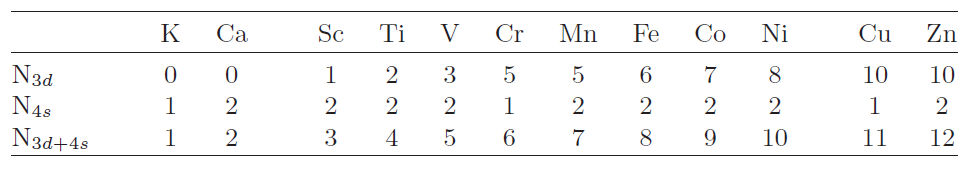
\includegraphics[width=150mm]{figs/TransitionMetalValenceShells}
	\end{center}
\caption{Number of 3d and 4s electrons in the free transition metal atoms}
\label{TransMetalUnpE}
\end{figure}

For example, in Fe, there is a possibility of 12 electrons occupying the 4s and 3d orbitals, and only 8 electrons occupying these positions, giving rise 4 unfilled "holes", for which situation Hund's rule would predict a magnetic spin moment of $\mu_s$=4$\mu_B$ for Fe, and similarly 3$\mu_B$ for Co and 2$\mu_B$ for Ni.

However, if the spontaneous magnetization M of Fe, Co and Ni is measured and divided by the number of atoms, the resulting values are $m_{exp}$ = 2.215 $\mu_B$ for Fe, 1.715 $\mu_B$ for Co, and 0.616 $\mu_B$ for Ni. The sizes of these values immediately illustrates that the atomic picture cannot provide an accurate description of the magnetism of solids. In the next section, we will take a different approach, accounting for the itinerant nature of the electrons, and treating the effects of bonding of the atoms in a metal lattice.

\subsection{Bragg scattering and Band structure}
Before we introduce a model that includes magnetism in the context of a crystalline lattice, we will first introduce the language of band structure and the effect of periodic boundary conditions on the solutions of Schr\"odinger's equation for electrons in a periodic potential such as a crystalline lattice of ions. We begin with Bragg reflection of the electron from the lattice.

The most important consequence of Bragg reflection in our discussion is that it leads to the presence of an energy gap. In the 1-D case, the Bragg equation becomes:
\begin{equation}
\begin{split}
2dsin\theta = n\lambda \\
k = n\pi/a
\end{split}
\end{equation}
The first reflection occurs at k = +/- $\pi$/a and the first energy gap is there as well. Other energy gaps occur for the other positive and negative integral values of n.

Reflection at k = +/-$\pi$/a arises because the wave reflected from the (p +/-1)st atom interferes constructively with the original wave at the pth atom. The region in k space between +/1 $\pi$/a is the first Brillouin zone.

At k = +/-$\pi$/a the stationary state wave functions are not traveling waves as for the free particle model, but the solutions at these particular k values are made up equally of waves traveling to the right and the left: standing waves.  For k = +/-$\pi$/a we have two independent standing wave solutions:
\begin{equation}
\begin{split}
\Psi_1 \approx sin(\pi x/a) \approx (e^{i\pi x/a}- e^{-i\pi x /a}) \\
\Psi_2 \approx cos(\pi x/a) \approx (e^{i\pi x/a}+ e^{-i\pi x /a})
\end{split}
\end{equation}

These solutions are made up of equal parts waves traveling to the right and left. Moreover, these solutions correspond to different values of the potential energy of the particle, owing to the positional shift between the two wavefunctions. $\Psi_1$ distributes charge preferentially midway between ion cores, while $\Psi_2$ distributes charge preferentially on the ion cores. On calculating average values of the potential energy over the three charge distributions, we expect the potential energy of $\Psi_1$ to be greater than that of a plane wave while that of $\Psi_2$ to be less than that of a plane wave.

If the potential energies of the states  $\Psi_1$ and $\Psi_2$ differ by an amount $\Delta$E, we have an energy gap  of width $\Delta$E. The physical reason for the gap is this: If wave functions at values of k far removed from the Brillouin zone boundaries +/- $\pi$/a may be represented by plane waves e$^{ikx}$, then in forming a solution of the wave equation as the boundaries are approached and Bragg reflection becomes imminent the wave gradually becomes an admixture of the wave e$^{i[k-(2\pi/a)]x}$ , until at the zone boundary k = +/-$\pi$/a and the solution is e$^{i\pi x/a}$ +/- e$^{-i\pi x /a}$. 

\subsection{The Stoner Model}
The problem of predicting the value of the magnetic moment for transition metals was solved by developing a band theory for magnetic systems, which was done in 1935 by Mott, Slater, and Stoner \cite{Slater1936,Slater1936a,Stoner1936,Heisenberg1937,Mott1935}. This model is called the Stoner model. 

In this model, the bonding interaction in the 3d electrons causes a smearing of the energy into a a band. The periodicity condition of the lattice leads to the characteristic periodic variations and as seen above, their band width increases with the inverse lattice constant. For our first description of the Stoner model, we can consider the average finite energy width of the valence band states and approximate the density of states as a simple semicircle as shown in Fig. \ref{StonerModel}.

\begin{figure}
	\begin{center}
		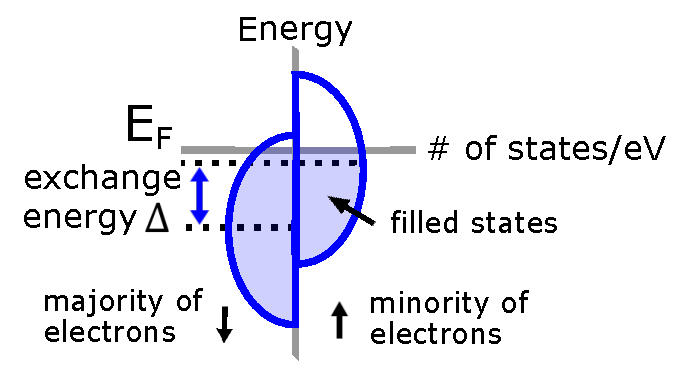
\includegraphics[width=100mm]{figs/StonerModel.pdf}
	\end{center}
	\caption{Stoner Model for ferromagnetic transition metals, and illustration of terms used for the description of this model. The filled electron states (at zero temperature) below the Fermi energy $E_F$ are shaded. The spin population with greater occupied states is called the majority band, while the population with less occupied states is called the minority band. The centers of the two bands are separated by the exchange energy $\Delta$.}
	\label{StonerModel}
\end{figure}

Here we introduce the terminology of majority and minority charge carriers. The electrons with spin states corresponding to the larger electron population are the "majority band" while those with the smaller population are the "minority band". This terminology will be extensively used in Section \ref{heuslerpaper}, since the distinction between minority and majority carriers becomes especially important for the special class of ferromagnets called half-metals studied in this project.

Next we proceed to derive an expression for the magnetic moment that is relevant for both electron and hole pictures. From the spin resolved density of states we can compute the number of spin states in the majority and minority bands by energy integration:
\begin{equation}
N_{e}^{maj}=N_e^\downarrow = \int_{-\inf}^{E_F}D^\downarrow(E)\text{d}E
\end{equation}

From electromagnetic theory, the atomic magnetic moment is given by m = -2$\mu_B$s/$\hbar$ with s having the units of [$\hbar$]. The absolute value of m can be found via the expectation of the electron spin operator $<s_z>$ according to the expression |m| = -2$\mu_B\braket{s_z}/\hbar$. Using the convention that the spin up states are labeled $\ket{\uparrow}$ = $\ket{+}$ with eigenvalue $s_z$ = +$\hbar$/2 and the spin down states $\ket{\downarrow}$ = $\ket{-}$ with eigenvalue $s_z$ = - $\hbar$/2, we have for $s_z$,
\begin{eqnarray}
\braket{s_z} = \braket{+\frac{1}{2}|s_z|+\frac{1}{2}}N_e^{min} + \braket{-\frac{1}{2}|s_z|-\frac{1}{2}}N_e^{maj} \\
= \frac{\hbar}{2}(N_e^{min}-N_e^{maj}) = \frac{\hbar}{2}(N_e^{\uparrow} - N_e^{\downarrow})
\end{eqnarray}
and we have the maximum number of electrons in the d shell: (2s+1)(2l+1) = 10. We also have $N_e$ + $N_h$ = 10. Thus  the number of holes in the minority band $N_h^{min}$ = $N_h^{\uparrow}$ and for the majority band $N_h^{maj}$ = $N_h^\downarrow$ is $N_e^\downarrow$ + $N_h^\downarrow$ = 5 and $N_e^\uparrow$ + $N_h^\uparrow$ = 5 and thus,
\begin{equation}
\braket{s_z} = \frac{\hbar}{2}(N_e^\uparrow-N_e^\downarrow) = -\frac{\hbar}{2}(N_h^\uparrow - N_h^{maj}).
\end{equation}
And finally we can conclude that the magnetic moment |m| is given by the difference in the number of electrons or holes in the majority and minority bands, according to
\begin{equation}
|m| = \mu_B(N_e^{maj}-N_e^{min}) = \mu_B(N_h^{min} - N_h^{maj}).
\end{equation}

When finally including these numbers, we find that in the band picture, the number of majority and minority states is a non-integer, and thus the magnetic moments are noninteger multiples of the Bohr magneton as experimentally measured. This simple relation between electron and hole moments is exact only if the band states are well defined in their energy spread about the Fermi level. In reality, there is hybridization between the d states and the s-p states such that even  10 eV above the Fermi level, there is some small d character in the s-p bands. Thus the number of d holes and the magnetic d moment is slightly reduced relative to the values expected from the filled electron states (cite stohr 240,241).

Since we now have a value for the magnetic moment, the exchange energy can also be written as an "exchange field", an effective magnetic field that splits the levels and can be used to describe the origin splitting as $\Delta$ = $2m\dot H_{ex}$. In addition, it exerts a torque T = $m\times H_{ex}$ on the electron spins. This gives us a surprisingly giant value for the effective exchange field of $10^3$ T. The size however gives us a quantitative understanding for the giant strength of the magnetic interaction in 3d ferromagnets. It is important to keep in mind that this exchange field does not act on the orbital moment or the nuclear magnetic moment, and thus the effect of the exchange interaction on the spin system is separate from the orbital system. The two systems can interact, but only via the (much weaker) spin-orbit interaction.

Although the Stoner model does a good job of predicting the magnetic moments of the transition metals by accounting for the bonds between atomic sites, there are some major shortfalls with the model. In particular, when attempting to calculate the Curie temperature for the transition metals, one comes up with a number several thousands of Kelvin higher than experimentally measured. This is because the Stoner model fails to account for interactions between electron spins directly. It is basically an extension of the Hubbard model to band theory rather than the Heisenberg model. In practice, a combination of the Stoner and Heisenberg models must be used in order to understand macroscopic behavior of ferromagnets.

\section{The next frontier: ultrafast laser-induced ferromagnet dynamics}

As a ferromagnetic metal approaches the Curie temperature, it reaches a critical point where the magnetic properties of the material change dramatically. Under equilibrium conditions, this ferromagnetic-to-paramagnetic phase transition is associated with critical phenomena, characterized by a vanishing of the spontaneous magnetization as well as a divergence of the magnetic heat capacity and susceptibility \cite{Stohr2006}. A faster route to change the magnetization is to use femtosecond laser irradiation: Since the first experimental observation of ultrafast laser- induced demagnetization \cite{E.BeaupaireJ-CMerleA.Daunois1996}, femtomagnetism has been a subject of intense experimental and theoretical studies. Although one might expect critical phenomena to play an important role in laser-induced de- magnetization of ferromagnetic metals, to date, there has been no clear evidence of this.

When a ferromagnetic metal is heated with a femtosecond laser pulse, the energy is directly coupled into the electron bath, creating an out-of-equilibrium electron distribution. This electron energy distribution quickly thermalizes (within tens of femtoseconds) to a hot Fermi-Dirac energy distribution. In most past work, the laser-induced demagnetization process is described as a sequence of events where the energy of the hot electron bath transfers first to the spin and later to the lattice degrees of freedom. This cascade of energy relaxation processes is used to explain why ultrafast demagnetization occurs over a range of time scales from 100 to 500 fs \cite{E.BeaupaireJ-CMerleA.Daunois1996,Koopmans2010}. These multiple time scales observed in past experiments obscured any contributions from critical phenomena. Although there is still no consensus on the important microscopic mechanisms that drive ultrafast demagnetization, or their relevant time scales, a number of microscopic models have been proposed. These are based on spin-flip scattering \cite{Koopmans2010, Zhang2009,Krauß2009,Bigot2009,Carpene2015,Mueller2013} that transfers spin angular momenta during the demagnetization process, as well as laser-induced polarized \cite{La-O-Vorakiat2012,Battiato2010,Rudolf2012} or unpolarized \cite{Dakovski2016,Eschenlohr2013} spin currents that can also lead to ultrafast demagnetization.

We note that the ability to manipulate the magnetic state on femtosecond timescales is important both scientifically and technologically. Although ferromagnetic metals are some of the simplest materials that exhibit strong interactions between the electron, spin, and lattice degrees of freedom, there is yet no comprehensive theory that describes their non-equilibrium behavior. Past work concluded that many different timescales were associated with laser-induced magnetic dynamics and that these depended on the pump fluence \cite{Tows2015,Illg2013} and sample geometry \cite{Schmidt2010, Turgut2016}. This made it challenging to develop complete theories and compare with experiments. In contrast, by showing the essential contribution of critical behavior associated with a magnetic phase transition, we reveal that only a few characteristic timescales are needed to fully explain ultrafast demagnetization in Ni.
